\newcommand{\leftimageheight}{4.5cm}
\newcommand{\rightimageheight}{4.5cm}

\renewcommand{\versionone}{
  \tikzsetnextfilename{blendfields_failures}
  \begin{tikzpicture}[
      >=stealth',
      overlay/.style={
          anchor=south west,
          draw=black,
          rectangle,
          line width=0.8pt,
          outer sep=0,
          inner sep=0,
        },
    ]
    \matrix[
      matrix of nodes,
      column sep=2pt,
      row sep=0pt,
      ampersand replacement=\&,
      inner sep=0,
      outer sep=0,
    ] (main) {
      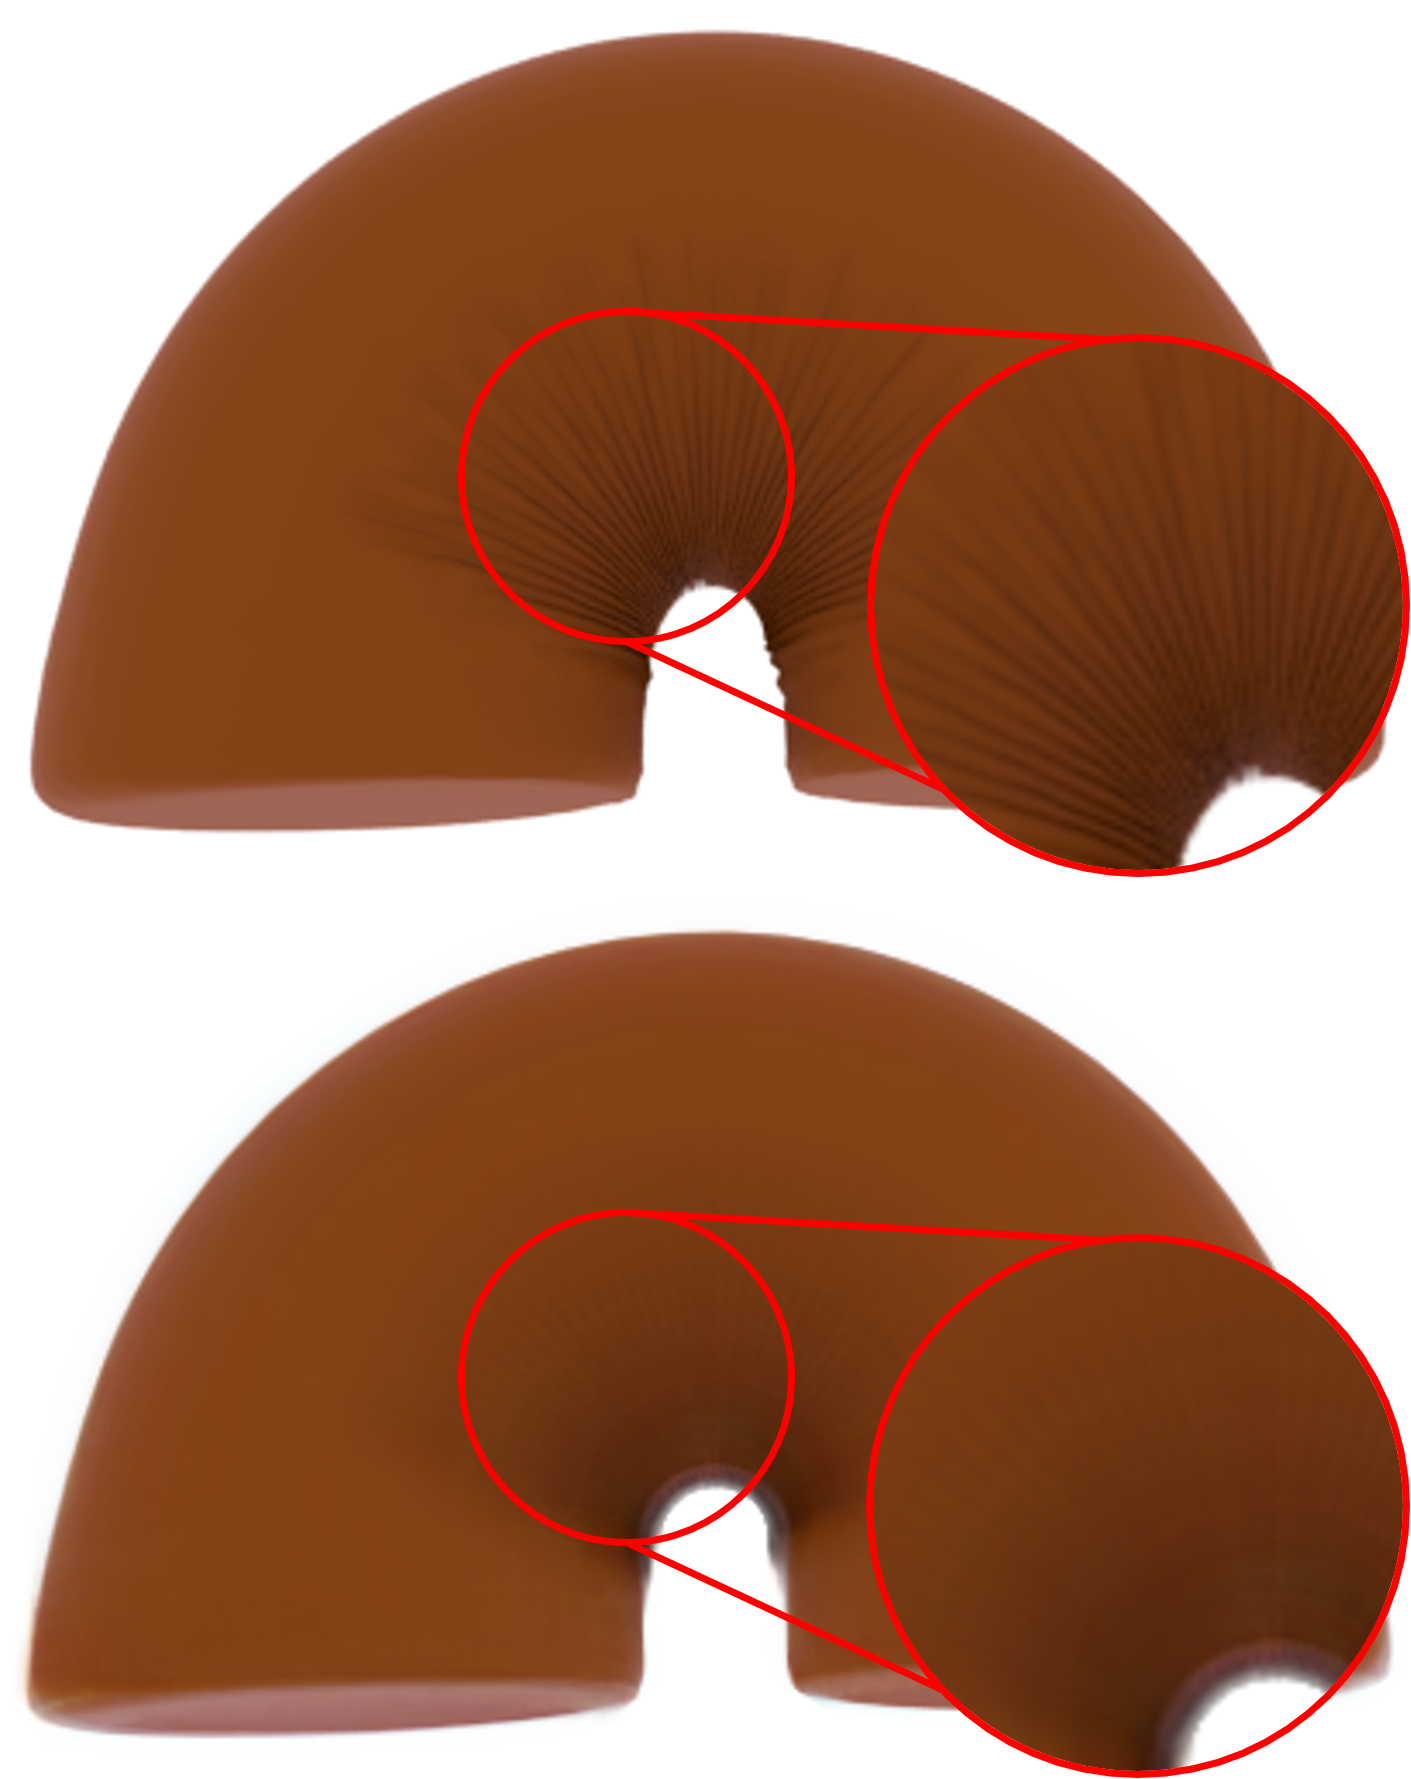
\includegraphics[height=\leftimageheight]{assets/\blendfieldsdirname/failures/convergence.png} \&
      \includegraphics[height=\rightimageheight]{assets/\blendfieldsdirname/failures/tracking.png} \\
    };
    \node[above=0.0em of main-1-1.north, align=center, anchor=south]{Low contrast};
    \node[above=0.0em of main-1-2.north, align=center, anchor=south]{Inaccurate off-the-shelf tracker};
  \end{tikzpicture}
}
\begin{figure}[t]
  \centering
  \resizebox{0.7\linewidth}{!}{\versionone}
  \caption{\textbf{Failure cases} -- {
      We show failure cases for our proposed approach.
      \textit{Left:}
      In the presence of wrinkles in low-contrast images, \blendfields takes
      longer to converge to make wrinkles visible.
      We show the ground truth on the top, and rendering after training
      $7{\times}10^5$ steps on the bottom.
      In contrast, we rendered images
      in~\cref{fig:blendfields-synthetic-qualitative} after $2{\times}10^5$
      steps.
      \textit{Right:} \blendfields inherits issues from VolTeMorph~\cite{garbin2024voltemorph}, which relies on the initial fit of the face mesh.
      If the fit is inaccurate, artifacts appear in the final render.
    }}
  \label{fig:blendfields-failure-cases}
\end{figure}